\chapter{Theory}

\section{Scientific Computing}

Scientific computing covers a large multi-disciplinary field, typically combining mathematics, computer science and engineering. For this project the most relevant subfield is High-Performance Computing (HPC) which focuses on high performance for short periods \cite{larsen:hpc}, in contrast to High-Throughput Computing (HPT) which focuses on finishing many tasks over a long period \cite{wisc:htcondor}. With the advent of big data, state of the art machine learning has begun intersecting more with the field of HPC.

HPC is typically done on clusters of computers with many CPUs and GPUs, connected through a high-speed communication bus. Workloads not designed for parallelism are not ideal to run on an HPC cluster, as HPC clusters do not perform single core processing particularly better than a server or desktop computer. Software is not perfectly paralellizable and there is always a part that has to be executed sequentially. Using Amdahl's Law \cite{larsen:hpc} in \eqref{eq:amdahl} it is possible to determine the maximum theoretical speedup for a piece of software, based on what percentage that is parallelizable. The variable $S$ means speedup and denotes how many times faster the software can be run as the amount of processors go to infinity. The value $p$ denotes the percentage of the program that is parallelizable and in practice it is impossible for it to be 1.

\begin{equation} \label{eq:amdahl}
    S = \frac{1}{1 - p}
\end{equation}

Figure \ref{fig:amdahl} shows Amdahl's Law for different values of $p$ with a $\log_2$ scaled x-axis. Although a $p$-value of 0.95 can double the speedup compared to a $p-value$ of 0.90, it also requires 4 times as many processors to reach its limit (512 vs. 2048 processors).

\begin{figure}[H]
    \centering
    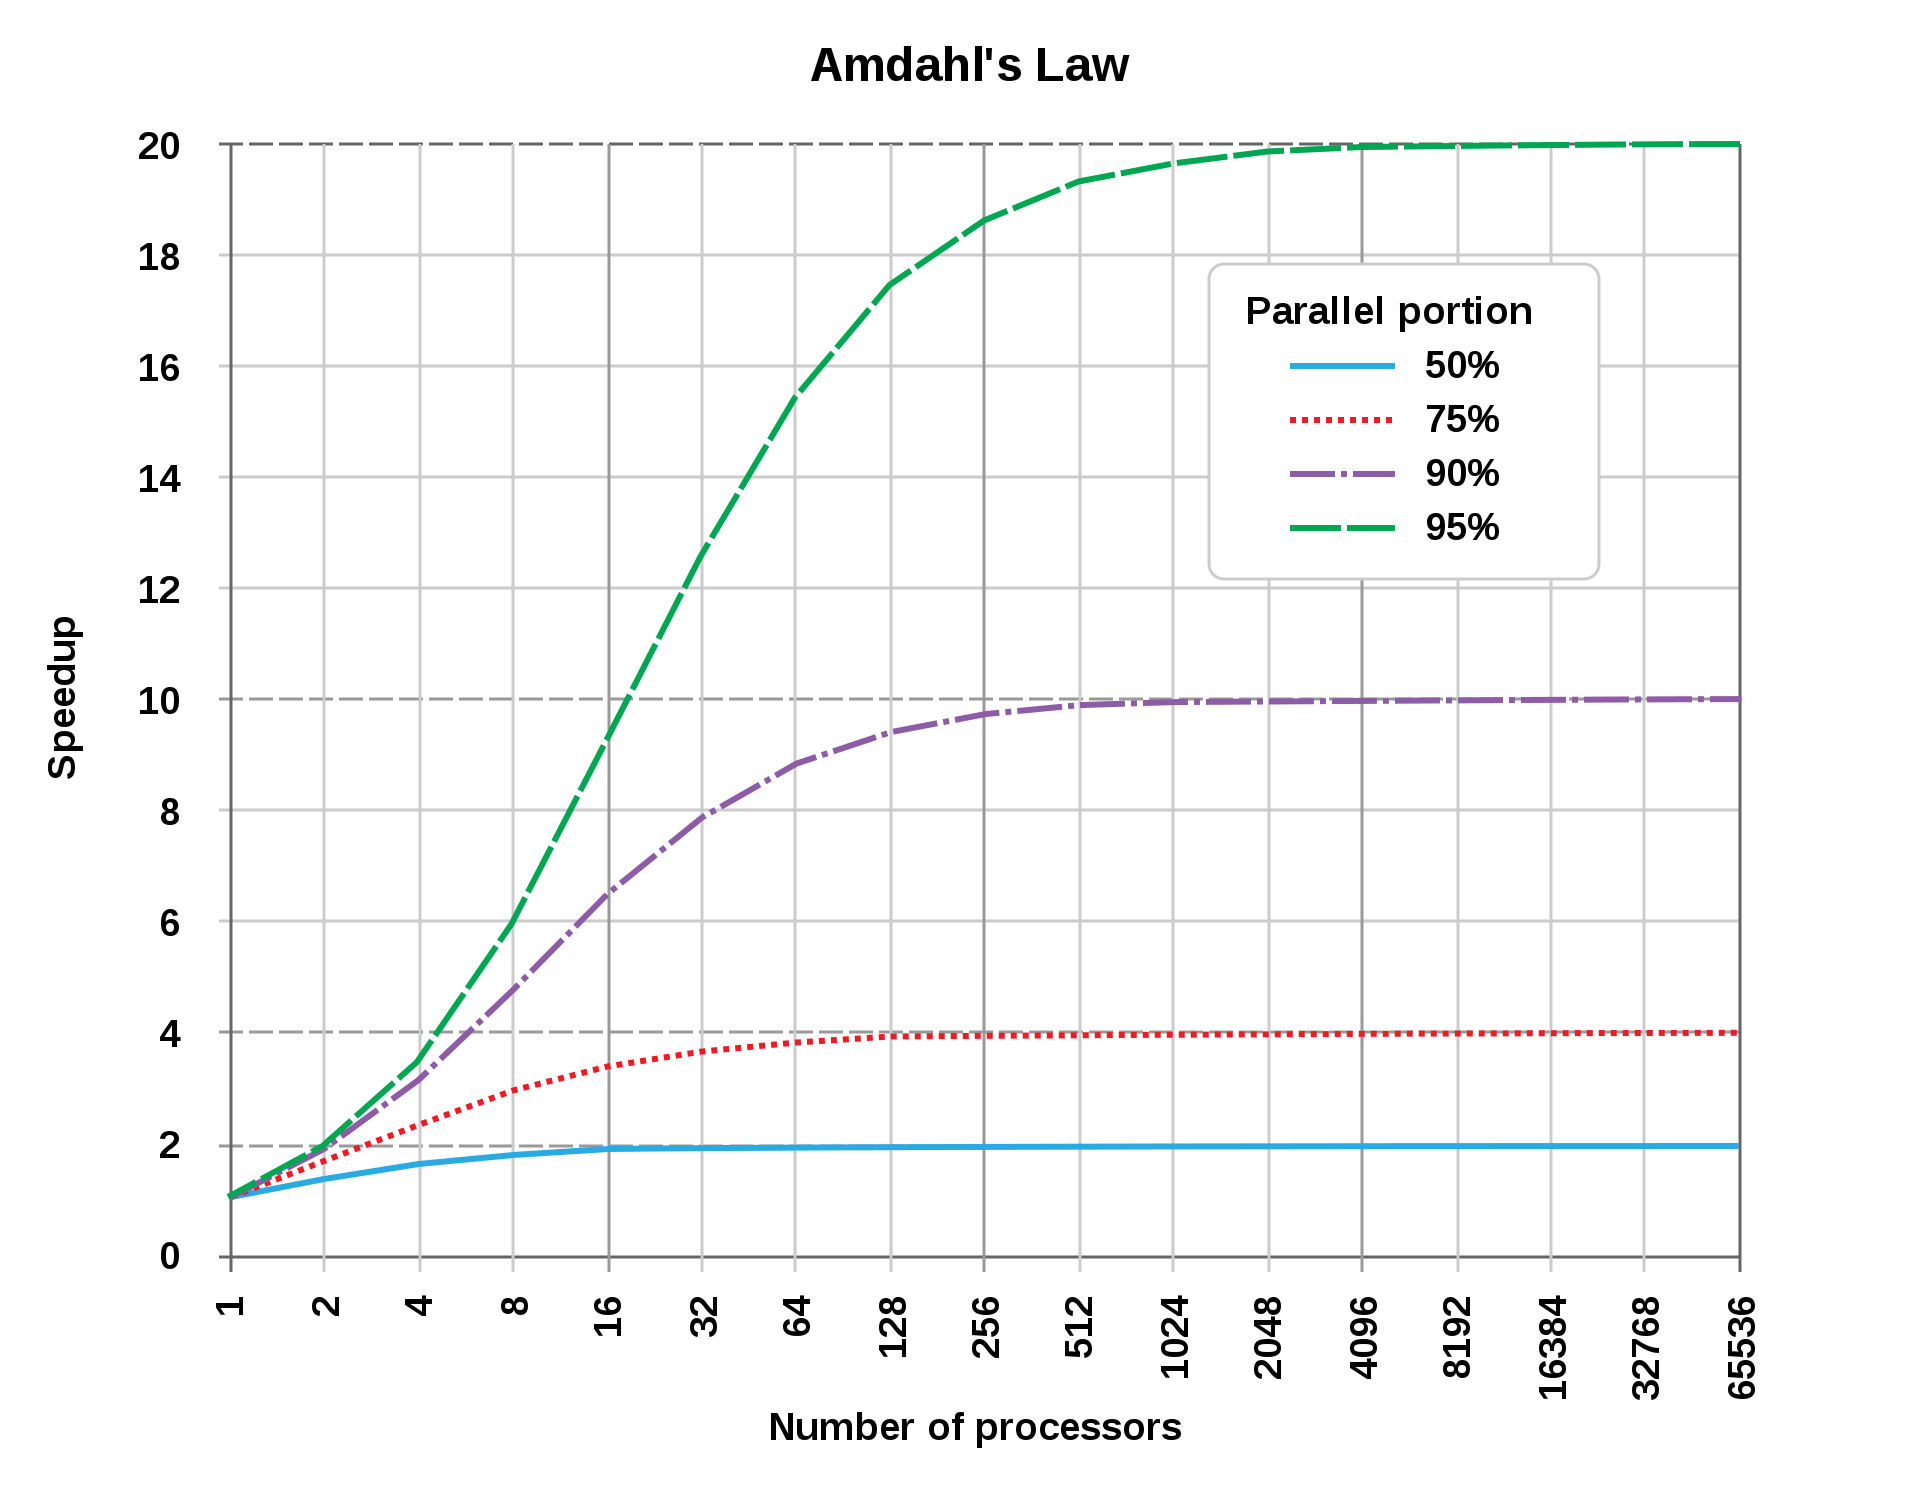
\includegraphics[scale=0.17]{Figures/amdahl.png}
    \caption[]{Amdahl's Law\protect\footnotemark\ with different percentage of parallelism}
    \label{fig:amdahl}
\end{figure} \footnotetext{\url{https://en.wikipedia.org/wiki/Amdahl\%27s\_law\#/media/File:AmdahlsLaw.svg}}

An alternative to Amdahl's law is Gustafson's Law, in \eqref{eq:gustafson}, which explicitely includes the number of processors. In Amdahl's Law $p$ is the percentage which is parallelizable, but in Gustafson's Law $s$ is used instead which is the percentage that is sequential (not parallelizable), thus $p = 1-s$.

\begin{equation}
  \label{eq:gustafson}
  S = N + (1 - N)s
\end{equation}

In theory it is simple to apply Amdahl's and Gustafson's Laws, but in practice it can be hard to determine exactly what percentage is and is not parallelizable. However they give insight into how a small non-parallelizable piece of code results in limited parallel performance as the amount of processors grow large. However, these laws do not give insight into the different types of parallelism.

To classify parallelism Flynn's Taxonomy is used.Figure \ref{fig:flynn:taxonomy} shows the different classifications of parallel computer architectures. The two most commonly used computer architectures in HPC are Single Instruction Multiple Data (SIMD) and Multiple Instruction Multiple Data (MIMD). The SIMD aspect in HPC comes from each CPU core and GPU being able to do data parallelism with their vector instructions. GPUs are typically able to compute more things in parallel than CPUs, but GPUs do not compute as many instructions per cycle (IPC) as a CPU. The MIMD aspect in HPC comes from combining multiple devices, which can be either multiple CPU cores, multiple GPUs or both.

\begin{figure}[H]
    \centering
    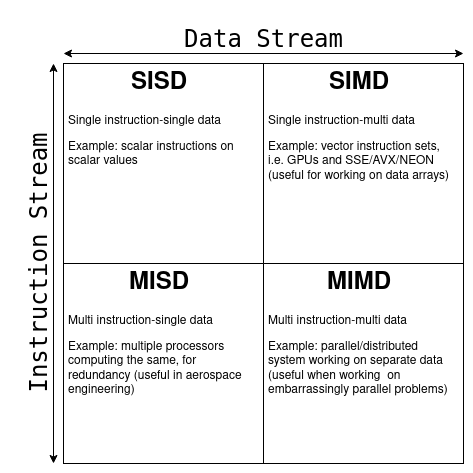
\includegraphics[scale=0.45]{Figures/flynns_taxonomy.png}
    \caption{Flynn's Taxonomy}
    \label{fig:flynn:taxonomy}
\end{figure}

To take advantage of the SIMD and MIMD architectures, libraries can be optimized to utilize multiple CPU cores, GPUs and/or vector instructions. The more popular libraries in HPC are the Basic Linear Algebra Subprograms (BLAS) specification, which specifies a specification for doing vector-vector, matrix-vector and matrix-matrix operations. The BLAS specification does not specify operations for matrix decomposition (i.e. SVD or EVD), but some libraries implementing BLAS also includes support for this.

The benefit of using these pre-existing linear algebra libraries is that a lot of time has already been spent on optimizing performance for their target platform. Intel and NVIDIA both make linear algebra libraries for their hardware platforms. Intel makes the \textit{Math Kernel Library} (MKL) which uses multiple cores and the vector instructions on their CPUs. NVIDIA makes the CUDA based \textit{cuBLAS} and \textit{cuSOLVER} libraries that are designed to run on one or more GPU. Both of these are designed for homogenous hardware, i.e. they cannot utilize both the CPU and GPU. Libraries like MAGMA are heterogeneous libraries, as they use CPU and GPU to compute different parts of a problem. MKL, cuBLAS/cuSOLVER and MAGMA are all MIMD based libraries, but they take advantage of the SIMD architecture of individual GPUs and CPU cores as they utilize vector instructions.

\section{Singular Value Decomposition}

The Singular Value Decomposition (SVD) is a very general matrix decomposition, which unlike the Eigenvalue Decomposition also works on non-square matrices. Given a matrix $X \in \mathbb{C}^{m \times n}$, the SVD results in the factorization in \eqref{eq:svd}. $U \in \mathbb{C}^{m \times m}$ and $V \in \mathbb{C}^{n \times n}$ are unitary matrices, and $S \in \mathbb{R}^{m \times n}$ is a diagonal matrix containing the singular values.

\begin{equation} \label{eq:svd}
    X = USV^T
\end{equation}

It is possible to compute the SVD by using Eigenvalue Decomposition using the relation between the two decompositions as in \eqref{eq:svd:evd1}. When $S$ and one of the unitary matrices has been computed, the other unitary matrix can be computed using the relation in \eqref{eq:svd:evd2}.
 
\begin{equation} \label{eq:svd:evd1}
\begin{split} 
    X^T X &= VSU^T USV^T = VS^T SV^T = V \Sigma_n V^T \\
    X X^T &= USV^T VS^TU^T = US S^TU^T = U \Sigma_m U^T
\end{split}
\end{equation}

\begin{equation} \label{eq:svd:evd2}
\begin{split} 
    U &= X V S^{-1} \\
    V &= X^T U S^{-1}
\end{split}
\end{equation}

This proves two important facts. The first is the singular values are the square root of the eigenvalues in $\Sigma_m$ and $\Sigma_n$. The second is that the singular value matrix $S$ is positive semi-definite, because $X^T X$ is positive semi-definite which has positive and real eigenvalues.

This method of calculating the SVD is inefficient for large matrices as solving the eigenvalue problem has a time complexity of $O(n^3)$ and matrix multiplication is done in $O(mn^2)$. To make it viable for larger matrices, there exists various parallel algorithms to calculate the SVD for both dense and sparse matrices \cite[Chapter~4]{erricos:handbook}. But with respect to calculating the \textit{score}, using any of these parallel SVD algorithms is not ideal as they calculate all the singular values, which is exactly what is not necessary.

There exists algorithms that can approximate the largest singular values of a matrix. It is possible to specify how many singular values that should be calculated. Two algorithms are the Randomized SVD (rSVD) and the Compressed SVD (cSVD). The rSVD is the older one and inspired Erichson, et. al. to make the cSVD \cite{erichson:csvd}. The cSVD is well suited for parallelization and it is also faster than the rSVD, therefore it makes sense to use the cSVD algorithm. The cSVD algorithm was originally made with image processing in mind, as it is well suited for computing the most significant singular values of sparse matrices. Because the EDJMs are also sparse when using ReLU activation functions, the cSVD should work for that specific problem too. To understand the idea behind the cSVD, it is necessary to understand the basics of compressed sensing.

\section{Compressed Sensing}

The basic idea behind compressive sensing is that higher dimensional sparse signals can be approximately reconstructed from lower dimensional signals. A sparse signal $X$ is sampled with the measurement matrix $\Phi$, resulting in the output signal $Y$ in \eqref{eq:compressive:vec} \cite{chen:mmv}. If $X$ is not sparse it is possible to use a basis transformation $\Psi$ to make it sparse. For instance, images are generally not sparse in the spatial domain but they are mostly sparse in the Fourier domain, so a potential basis transformation is a 2-dimensional DFT.

\begin{equation} \label{eq:compressive:vec}
\begin{split}
    Y = \Phi X &, \ \mathrm{where}      \\
    X &\in \mathbb{C}^{N \times L}      \\
    \Phi &\in \mathbb{C}^{m \times N}   \\
    Y &\in \mathbb{C}^{m \times L}      \\
    N &\gg m
\end{split}
\end{equation}

To measure how sparse a matrix is, the rank sparsity measure is used \cite{chen:mmv}. This measure is shown in \eqref{eq:sparsity:measure}. In this context $x_i$ are the transposed row vectors of $X$ .

\begin{equation} \label{eq:sparsity:measure}
  \begin{split}
      X &= [x_1\ x_2 \cdots x_N]^T \\
      m(x_i)_{N \times 1} &= [||m(x_1)||_p\ ||m(x_2)||_p\ \cdots ||m(x_N)||_p]^T,\quad p \in \mathbb{N}\setminus 0
  \end{split}
\end{equation}

Because $Y = \Phi X$ is an underdetermined problem, there are an infinite amount of solutions to it. Compressive sensing uses the sparsity the signal $X$ and makes the argument that a very good solution to the underdetermined problem must be the most sparse solution. This can be specified as the minimization problem in \eqref{eq:compressive:l0}, which minimizes the rank sparsity of $X$ \cite{chen:mmv}. Minimizing the rank sparsity is an NP-hard problem, which makes it unfeasible in real applications.

\begin{equation} \label{eq:compressive:l0}
  \min_{X} || (m(x_i))_{N \times 1} ||_0 \quad s.t. \quad Y = \Phi X
\end{equation}

It is possible to relax the problem, transforming it from a combinatiorial non-convex problem to a convex problem. This is done by using the $l1$-norm instead of the $l0$-norm as shown in \eqref{eq:compressive:l1} \cite{chen:mmv}. It's important to note that the relaxation does not guarantee optimal reconstruction as the original optimization problem. 

\begin{equation} \label{eq:compressive:l1}
    \min_{X} || (m(x_i))_{N \times 1} ||_1 \quad s.t. \quad Y = \Phi X
\end{equation}

To determine how well the relaxed reconstruction works based on the measurement matrix $\Phi$ works, the mutual coherence, in \eqref{eq:mut:coherence} can be computed \cite{chen:mmv}. The best case is complete incoherency, when the mutual coherence is 0. In this case the relaxed problem and the optimal problem provide the same result. As the mutual coherence of $\Phi$ increases, the chances of optimal reconstruction decreases.

\begin{equation} \label{eq:mut:coherence}
    \mu(\Phi) = \max_{1 \le i \neq j \le L} | G_{i,j} |,\quad G = \Phi\Phi^H
\end{equation}

Usually, in compressed sensing problems, only the output signal $Y$ and the measurement matrix $\Phi$ are known, therefore the goal is to estimate $X$ in the underdetermined problem in \eqref{eq:compressive:l0}. But for the cSVD $Y$, $\Phi$ and $X$ are already known beforehand, and thus it becomes a problem of estimating a low rank approximation of $X$ based on $Y$ and $\Phi$ rather than finding the sparsest $X$ for $Y = \Phi X$.

\section{Compressed Singular Value Decomposition}

The cSVD algorithm, in Algorithm \ref{alg:csvd}, takes inspiration from compressed sensing, it is based on the idea of random sampling and with the intent of minimizing the norm of a matrix as in \eqref{eq:csvd:min}, where $X$ is the input matrix and $X_k$ is the low-rank approximation using $k$ singular values.

\begin{equation}
  \label{eq:csvd:min}
  \min_{\hat X_k} || X - \hat X_k ||_F
\end{equation}

\begin{algorithm}[H]
  \label{alg:csvd}
\SetAlgoLined
\SetKwInOut{Input}{Input}
\Input{Sparse matrix $X \in \mathbb{R}^{m \times N}$, target rank k and oversampling p}
$l \gets k + p$ \\
$\Phi \gets \mathrm{rand}(l, m)$ \\
$Y \gets \Phi X$ \\
$B \gets Y Y^T$ \\
$B \gets \frac{1}{2}(B + B^T)$ \\
$T,D \gets \mathrm{eigs}(B,k)$ \\
$\tilde S \gets \sqrt{D}$ \\
$\tilde V \gets Y^T T \tilde S^{-1}$ \\
$\tilde U \gets X \tilde V$ \\
$U,S,Q^T \gets \mathrm{svd}(\tilde U)$ \\
$V \gets \tilde V Q$ \\
\KwResult{$U \in \mathbb{R}^{m \times k}$, $S \in \mathbb{R}^{k \times k}$, $V \in \mathbb{R}^{n \times k}$}
\caption{cSVD}
\end{algorithm}

$ $ \newline

The time complexity of the cSVD algorithm is dominated by the computation of $\tilde U \sim O(mnk)$. The only computation coming close in time complexity is $\mathrm{svd}(\tilde U) \sim O(mk^2)$. The naïve SVD is in $O(n^3)$ while a better algorithm such as a QR based SVD is in $O(mn^2)$. If the largest 10\% singular values are desired, it results in a tenth of the computation when comparing $O(mnk)$ and $O(mn^2)$.

One way to optimize the algorithm is to choose a good $\Phi$. Erichson, et. al. mentions a Gaussian matrix works well \cite{erichson:csvd}. An argument for this is because the rows are linearly independent, with high probability, which results in a lower mutual coherence. The downside is Gaussian matrices are computationally intensive to generate.

By using the fact that during DNN training the training data is shuffled, it is possible to use a more efficient and deterministic $\Phi$. By collecting the first $l$ rows from an EDJM, assuming the trainng data is shuffled every epoch, it corresponds to using a $\Phi$ with linearly independent rows that are all unique standard basis vectors. The example in \eqref{eq:phi:example} shows a $\Phi$ sampling three random rows from an EDJM that has five rows, assuming no data is being shuffled. A value of $1$ in $(3,2)$ results in the second row of the EDJM ending up in the third row of the sampled EDJM matrix. $\Phi$ in this case is practically a permutation matrix with lots of zero columns.

\begin{equation} \label{eq:phi:example}
    \Phi =
    \begin{bmatrix}
    1 & 0 & 0 & 0 & 0 \\
    0 & 0 & 1 & 0 & 0 \\
    0 & 1 & 0 & 0 & 0
    \end{bmatrix}
  \end{equation}

Calculating the coherence, as in \eqref{eq:mut:coherence}, for a $\Phi$ that is this type of permutation matrix is simple because the zero columns can be removed. This means the mutual coherence is computed for a permutation matrix with its transpose. A permutation matrix multiplied with its transpose always results in an identity matrix. The identity matrix does not have any indices for $i \neq j$ that is non-zero. Therefore the coherence results in zero, which is the best possible case.
